\chapter{NVARs in Practice}\label{ch:nvar-application}

In this chapter, I will resolve the practical questions raised in
\cref{ch:nvar}, and demonstrate that NVARs are capable of solving
traditional RC problems well with very few taps, simple
nonlinearities, and very little training data. Using the example
systems from \cref{ch:systems}, I will use NVARs to perform state
inference and forecasting on the Lorenz '63 system, forecasting on the
double-scroll circuit, and forecasting on the Mackey-Glass time-delay
system.

The work presented in this chapter is the result of a
collaboration\cite{gauthier2021}. My contribution involves the initial
implementation and exploration of the NVAR method, discussion during
the development of the Lorenz '63 results, as well as the
implementation of the Lorenz return map, double-scroll forecasting,
and Mackey-Glass forecasting.

\section{State Inference with Lorenz '63}

For this inference task, we provide an NVAR with the $x$ and $y$
components of the Lorenz '63 system, and train it to infer the third
$z$ variable. Inference tasks like this are useful in situations where
some variables of a system are easily measureable, while the rest are
only measureable with great care or expense. An NVAR or RC can be
trained on a short recording of the full state of the system, and then
used later to infer the difficult variables from the easy ones.

For this task, we use an integration timestep of $\Delta t = 0.05$. To
build an NVAR, we must choose the tap delays $\tau_i$, the
nonlinearity $\bm{g}_\text{n}$, and ridge parameter $\alpha$. Takens'
embedding theorem\cite{takens1981} provides guidance on the expected
number of taps: as the dimension of the Lorenz attractor is slightly
larger than $2$, we choose to use $4$ equally spaced taps $\tau_0 =
0$, $\tau_1 = 5$, $\tau_2 = 10$, and $\tau_3 = 15$. These taps are
spaced to equally cover roughly one Lyapunov period, with the last tap
at time $\Delta t \tau_3 = 0.75$.

For the non-linearity $\bm{g}_\text{n}$, we use a slightly modified
version of the quadratic output introduced in
\cref{eq:quadratic-nvar}. This $\bm{g}_\text{n}$ includes a constant
term, all linear terms of the tap vector $\bm{x}$, and all quadratic
terms of the tap vector $\bm{x}$. That is,
\begin{equation}
  \label{eq:quadratic-nvar-const}
  \bm{g}_\text{n}(\bm{x}) = [1, x_1, x_2, \dots, \; x_1 x_1, x_1 x_2, \dots, \; x_2, x_2, \dots].
\end{equation}
The addition of a constant term allows the trained linear
$W_\text{out}$ to fit a constant offset, which is useful here as the
$z$ component has a non-zero mean.

For this task, with $4$ taps and two input dimensions $x$ and $y$, the
output of $\bm{g}_\text{out}$ has $45$ components, and the linear
output matrix $W_\text{out}$ has dimension $1 \times 45$.

\begin{figure}
  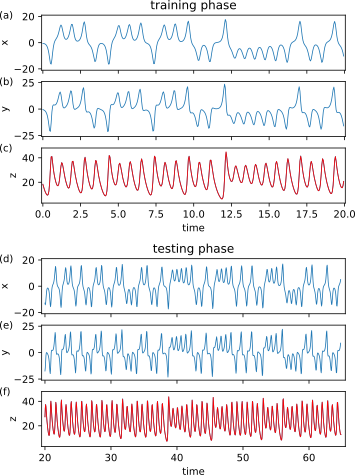
\includegraphics{figures/nvar-infer-lorenz}
  \caption{(a) -- (c) The Lorenz '63 system (blue) during the NVAR
    training. After the NVAR is trained, it can be re-used on the
    training signal to produce the training output (c, red). (d) --
    (f) The Loenz '63 system during NVAR testing, with the NVAR
    output. In both cases, the NVAR output (red) lies directly on top
    of the true Lorenz signal (blue).}
  \label{fig:nvar-infer-lorenz}
\end{figure}

We train this NVAR on $10$ different examples of the Lorenz '63
system, using $x$ and $y$ as the example input and $z$ as the example
output. Each training example is $20$ units of time. We then evaluate
the NVAR for $45$ units of time to produce a NRMSE $\epsilon$ as in
\cref{eq:nrmse}, and then average these errors over all $10$
trials. During evaluation, the NVAR has access to only $x$ and $z$,
and must produce an estimate of $z$. We then adjust $\alpha$ manually
to minimize this error. This whole process, training the NVAR $10$
different times and evaluating the error, takes only a few seconds on
a modern computer, even with a poorly-optimized implementation.

We find this NVAR has a NRMSE of $1.75\mp0.3\times10^{-2}$ on this
inference task, with $\alpha = 0.05$. An example of the NVAR during a
single training and testing trial is shown in
\cref{fig:nvar-infer-lorenz}.

\section{Forecasting Lorenz '63}

For this task, we will use an NVAR in forecasting mode to do system
forecasting for Lorenz '63. That is, we train the NVAR to use all
three state variables $x$, $y$, and $z$ to perform next-step-ahead
prediction of the Lorenz system. Unlike for the inference task, once
the NVAR is in forecast mode it no longer has an external driving
input and runs autonomously. As a result, the choice of time step
$\Delta t$ has a stronger effect on forecasting than inference. Too
small a time step is wasted effort, and too large risks
innacuracy. Here, we use a time step of $\Delta t = 0.025$.

Again we use the quadratic non-linearity with constant term described
in \cref{eq:quadratic-nvar-const}. In this case, the non-linear output
of $\bm{g}_\text{out}$ has $28$ components, and so $W_\text{out}$ has
dimension $3 \times 28$.

For the forecasting task we use only $2$ taps, $\tau_0 = 0$ and
$\tau_1 = 1$. This effectively gives the NVAR access to the current
value of the input as well as its derivative, and we find this
entirely sufficient for the forecasting task.

Again, we train this NVAR on $10$ different examples of the Lorenz '63
system, each time training on $10$ units of time. We then evaluate the
NVAR by performing an autonomous forecast for one Lyapunov period to
calculate a NRMSE $\epsilon_1$, as in \cref{eq:nrmse}, and then
average this over the $10$ trials to produce $\tilde{epsilon}$ in
\cref{eq:nrmse-avg}.

\begin{figure}
  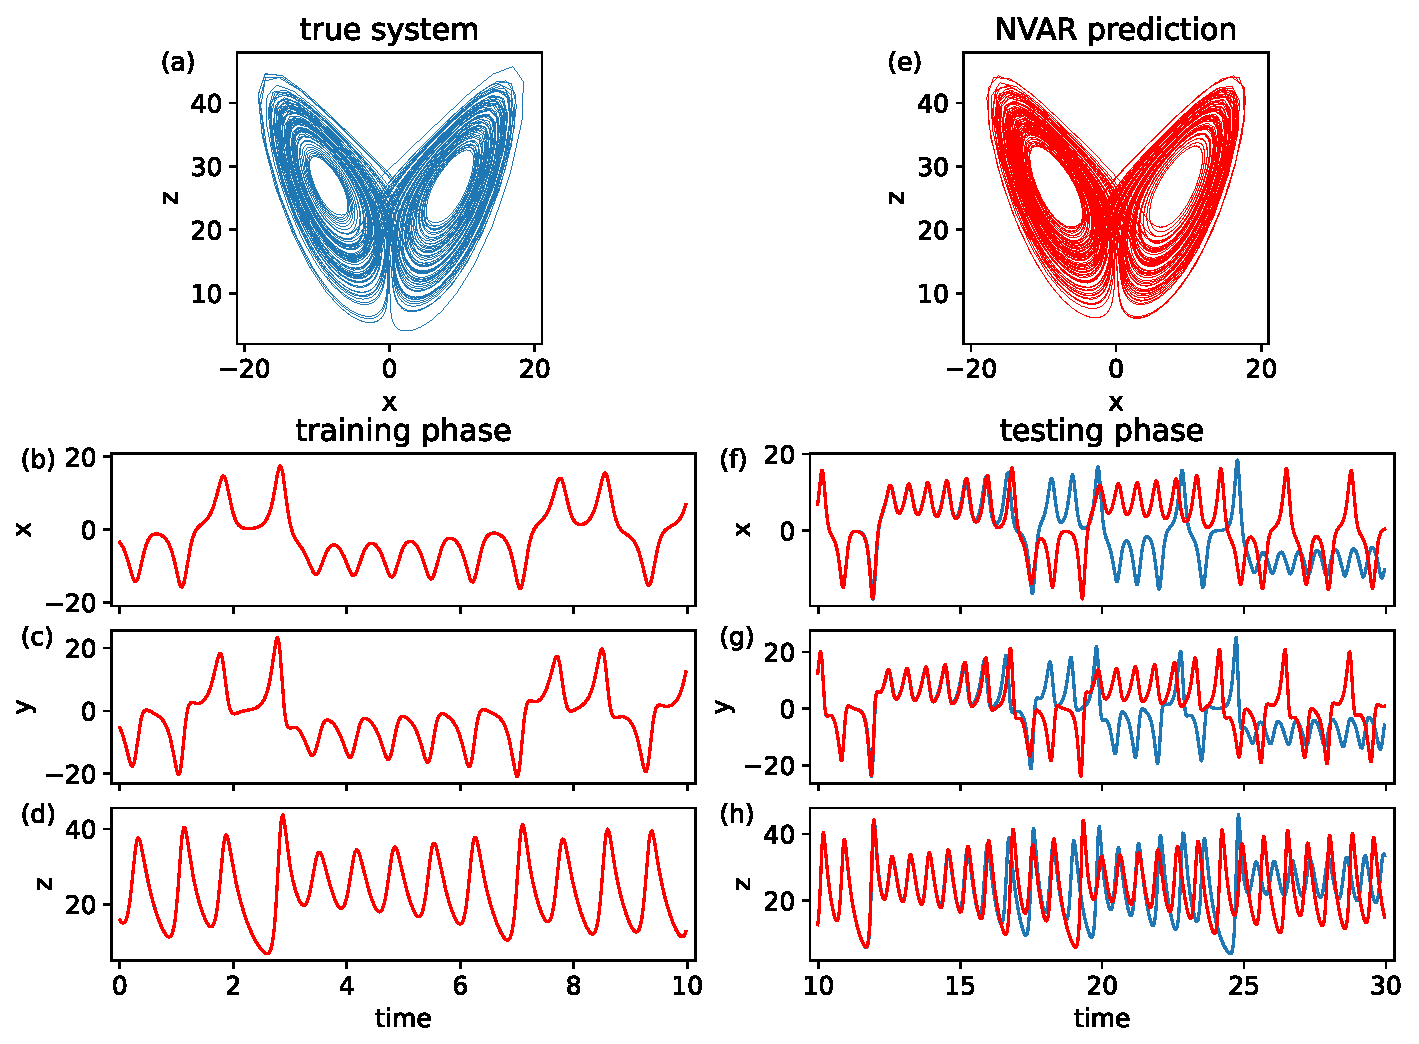
\includegraphics[width=\textwidth]{figures/nvar-predict-lorenz}
  \caption{The true Lorenz attractor (a) and NVAR predicted attractor (b) for a single training trial. (b) -- (d) True Lorenz system (blue) during training overlaid with NVAR output (red) calculated after training is complete. (f) -- (h) True (blue) and NVAR forecasted output (red).}
  \label{fig:nvar-predict-lorenz}
\end{figure}

The performance of this NVAR during a single training trial is shown
in \cref{fig:nvar-predict-lorenz}. A long autonomous forecast from the
NVAR produces an attractor that shows qualitative agreement with the
true Lorenz attractor, and produces a NRMSE over one Lyapunov period
of $2.32\pm0.51\times10^{-3}$, about ten times better than the ESNs
described in \cref{tab:lowk-lorenz-results}. This NVAR performs better
than the ESNs despite the fact that they are simpler to describe and
implement, do not require lengthy optimization, and train at least an
order of magnitude faster. The training data used for the NVAR is also
very light: only $10$ units of time, corresponding to $400$ points at
this time step, is sufficient to train the NVAR this well.

The $z$ variable of the Lorenz '63 system has a functional relation
between successive local maxima. This is demonstrated visually by
finding the local maxima $z_i$ of $z$, and then plotting $z_i$ with
respect to $z_{i+1}$ \cite{lorenz1963}. This \emph{return map} neatly
summarizes the long-term behavior of the $z$ variable, and comparing
two such maps provides a quick way to qualitatively compare two
systems. This comparison has been used previously to verify that a
trained RC can replicate the Lorenz '63 dynamics. \cite{pathak2017}

In many ways, this comparison is like the visual inspection of the
reproduced attractor in \cref{fig:nvar-predict-lorenz}. However, the
return map is a much simpler shape and is much more sensitive to error
than the attractor itself even when comparing two maps by eye. Indeed,
the return map is so sensitive that it depends the specific integrator
used to find the true Lorenz '63 solution. Here, we use an explicit
Runge-Kutta 3(2)\cite{dormand1980} integrator for both the Lorenz '63
and double-scroll systems.

The values of the maxima in the discrete-time solutions for both the
NVAR and Lorenz '63 system depend on the time step $\Delta t$ used for
integration, as the true maximum may be achieved in between the
discrete time steps. To better reproduce the true Lorenz '63 return
map, and to reduce the effect $\Delta t$ has on the NVAR return map,
we interpolate the $z$ solutions by using a degree-$4$ spline. The
local maxima are then found on this interpolated spline.\cite{dierckx1995}

\begin{figure}
  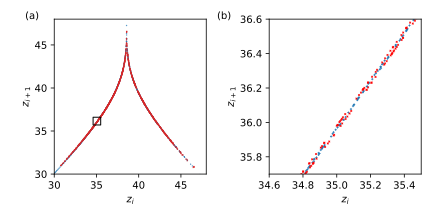
\includegraphics{figures/nvar-lorenz-rmap}
  \caption{(a) The $z$ return map of the Lorenz '63 system (blue $+$)
    overlaid with the $z$ return map of the NVAR forecast (red
    $\times$). The NVAR reproduces the long-term dynamics of the $z$
    variable accurately enough at this scale that it is difficult to
    see the true return map underneath. (b) Detail of the region
    marked in (a). At this scale, it is possible to see the small
    difference between the true and predicted return maps.}
  \label{fig:nvar-lorenz-rmap}
\end{figure}

\Cref{fig:nvar-lorenz-rmap} shows the return maps for both the true
Lorenz system and the NVAR. Qualitatively, there is good agreement
between the two. The NVAR return map almost completely obscures the
true Lorenz return map at this scale. Upon close inspection, we see
that the NVAR return map does not line up precisely with the true
return map. This can be improved by extending the training time of the
NVAR, but the difference between the two return maps is already small
even when the NVAR is trained for only $10$ units of time.

As with the attractor comparison, a quantitative measure of return map
similarity would be a strong candidate for replacing the flawed NRMSE
measure.

% fixed points discussion
% wout discussion

\begin{figure}
  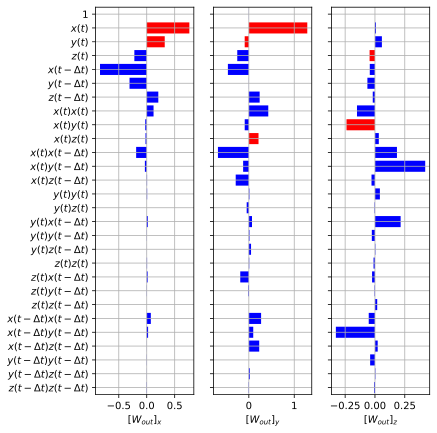
\includegraphics{figures/nvar-predict-lorenz-wout}
  \caption{FIXME caption.}
  \label{fig:nvar-predict-lorenz-wout}
\end{figure}

\section{Forecasting the Double-Scroll Circuit}

\begin{figure}
  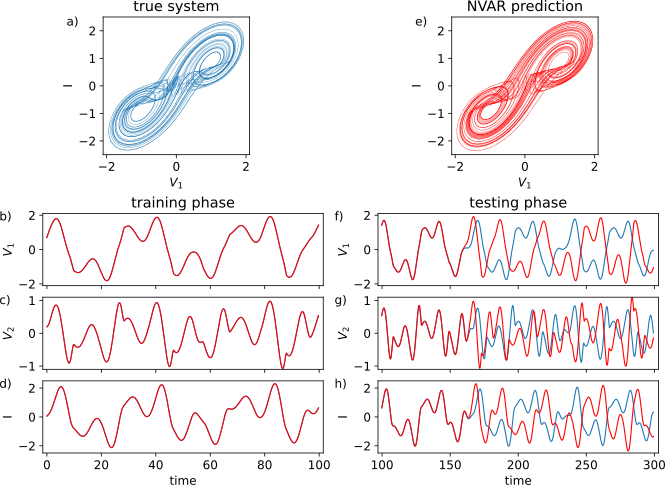
\includegraphics[width=\textwidth]{figures/nvar-predict-dscroll}
  \caption{FIXME caption.}
  \label{fig:nvar-predict-dscroll}
\end{figure}

\section{Forecasting Mackey-Glass}

\begin{figure}
  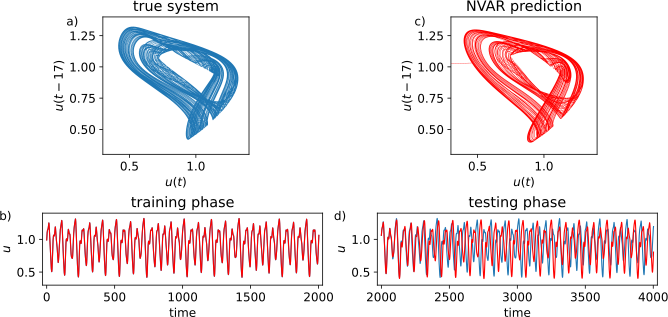
\includegraphics[width=\textwidth]{figures/nvar-predict-mackey-glass}
  \caption{FIXME caption.}
  \label{fig:nvar-predict-mackey-glass}
\end{figure}
